% !TEX root =  ../Dissertation.tex

\chapter{Data and Experimental Setup}
\label{ch:setup}
This chapter describes which data I take and how I process it, and how everything is set up. This includes the two chosen universes, the market-level signals I am considering, the hyperparameters of the reservoir, initialization of training heads, and the strict reproducibility discipline that every experiment in Chapter~\ref{ch:results} obeys. 

\section{Universes and calendars}
\label{sec:universes}

For the universe, I needed something that has relatively fixed inputs over time because the reservoir is static and can only have a fixed number of inputs. If we chose, say, the Dow 30, then since it keeps changing, taking the current top values would introduce confirmation bias. Thus, I choose two universes and further select them so they are deliberately different in character. The first, \texttt{etf10}, is a cross-asset universe of ten exchange-traded funds spanning equities, gold, commodities, treasuries, etc. It has obvious safe assets so a model can express a risk-off view by rotating into, say, bonds or gold. The second, \texttt{sector11}, is the eleven S\&P~500 sector funds, an all-equity universe with no obvious defensive asset. Then I added cash to both for realism and as a risk-free option. Table~\ref{tab:universes} lists both the universes except the cash column.


\begin{table}[t]
  \centering
  \begin{minipage}[t]{0.48\textwidth}
    \centering
    \textbf{\texttt{etf10}} (cross-asset, from 2006)\\[2pt]
    \begin{tabular}{ll}
      \hline
      Ticker & Exposure \\
      \hline
      SPY & US large-cap equity \\
      IWM & US small-cap equity \\
      VGK & European equity \\
      EEM & Emerging-market equity \\
      TLT & Long Treasuries \\
      IEF & Intermediate Treasuries \\
      LQD & Investment-grade credit \\
      DBC & Commodities \\
      GLD & Gold \\
      VNQ & US real estate \\
      \hline
    \end{tabular}
  \end{minipage}
  \hfill
  \begin{minipage}[t]{0.48\textwidth}
    \centering
    \textbf{\texttt{sector11}} (all-equity, from 1999)\\[2pt]
    \begin{tabular}{ll}
      \hline
      Ticker & Sector \\
      \hline
      XLE & Energy \\
      XLF & Financials \\
      XLK & Technology \\
      XLV & Health Care \\
      XLY & Consumer Discretionary \\
      XLP & Consumer Staples \\
      XLI & Industrials \\
      XLB & Materials \\
      XLU & Utilities \\
      XLRE & Real Estate (2015) \\
      XLC & Communication Services (2018) \\
      \hline
    \end{tabular}
  \end{minipage}
  \caption{The two universes. Every universe also carries a CASH column earning
  the risk-free rate. Two sector funds enter late and are handled by the
  availability matrix.}
  \label{tab:universes}
\end{table}

The two universes are kept entirely separate; they are never used together in any analysis. Additionally they run on different calendar since  \texttt{etf10} stated in February 2006 while \texttt{sector11}
started from January 1999, and they are different kinds of testbeds. This gives us richer context than if we were to club them together, which would also lead to the same fixed-reservoir input issue discussed above. To build the trading calendar, I take the union of days on which at least one asset is traded; this creates no dependency and thus no point of failure, except for the API that provides the trading days.

Two of the sector funds, XLRE and XLC, did not exist at the start of the sample, they enter in October 2015 and June 2018 respectively. This causes the fixed input issue. Thus I only give it the assets that are present at the inception to the reservoir but on readout I do that to the full final asset values, but this can lead to buying an asset that does not even exist yet, to resolve this I introduce the availability matrix. The availability matrix $A \in \{0,1\}^{T \times N}$ records which assets are tradeable on each day. For asset $i$, let $\tau_i$ and $\omega_i$ be its first and last observed trading days. Then
\begin{equation}
  A_{t,i} =
  \begin{cases}
    1 & \text{if } \tau_i \le t \le \omega_i,\\
    0 & \text{otherwise,}
  \end{cases}
  \label{eq:availability}
\end{equation}
so an asset is available for its whole active life; an interior missing print does not remove it, because the asset still existed that day. The matrix is turned into an additive logit mask,
\begin{equation}
  m_{t,i} = \big(1 - A_{t,i}\big)\,(-10^{9}),
  \label{eq:logit-mask}
\end{equation}
which is $0$ where available and $-10^{9}$ where not. A masked expert then outputs $w_t = \operatorname{softmax}(z_t + m_t)$, and $\exp(z_{t,i} - 10^{9})$ underflows to exactly $0$, so an unavailable asset receives precisely zero weight

Figure~\ref{fig:coverage} shows the resulting coverage. The final eighteen months, 1~January 2025 to 30~June 2026, are held out: they are removed from every artifact as it is loaded, and a guard raises an error if any evaluation window crosses that boundary, so those dates are absent from memory in all but the single holdout run.

\begin{figure}[t]
  \centering
  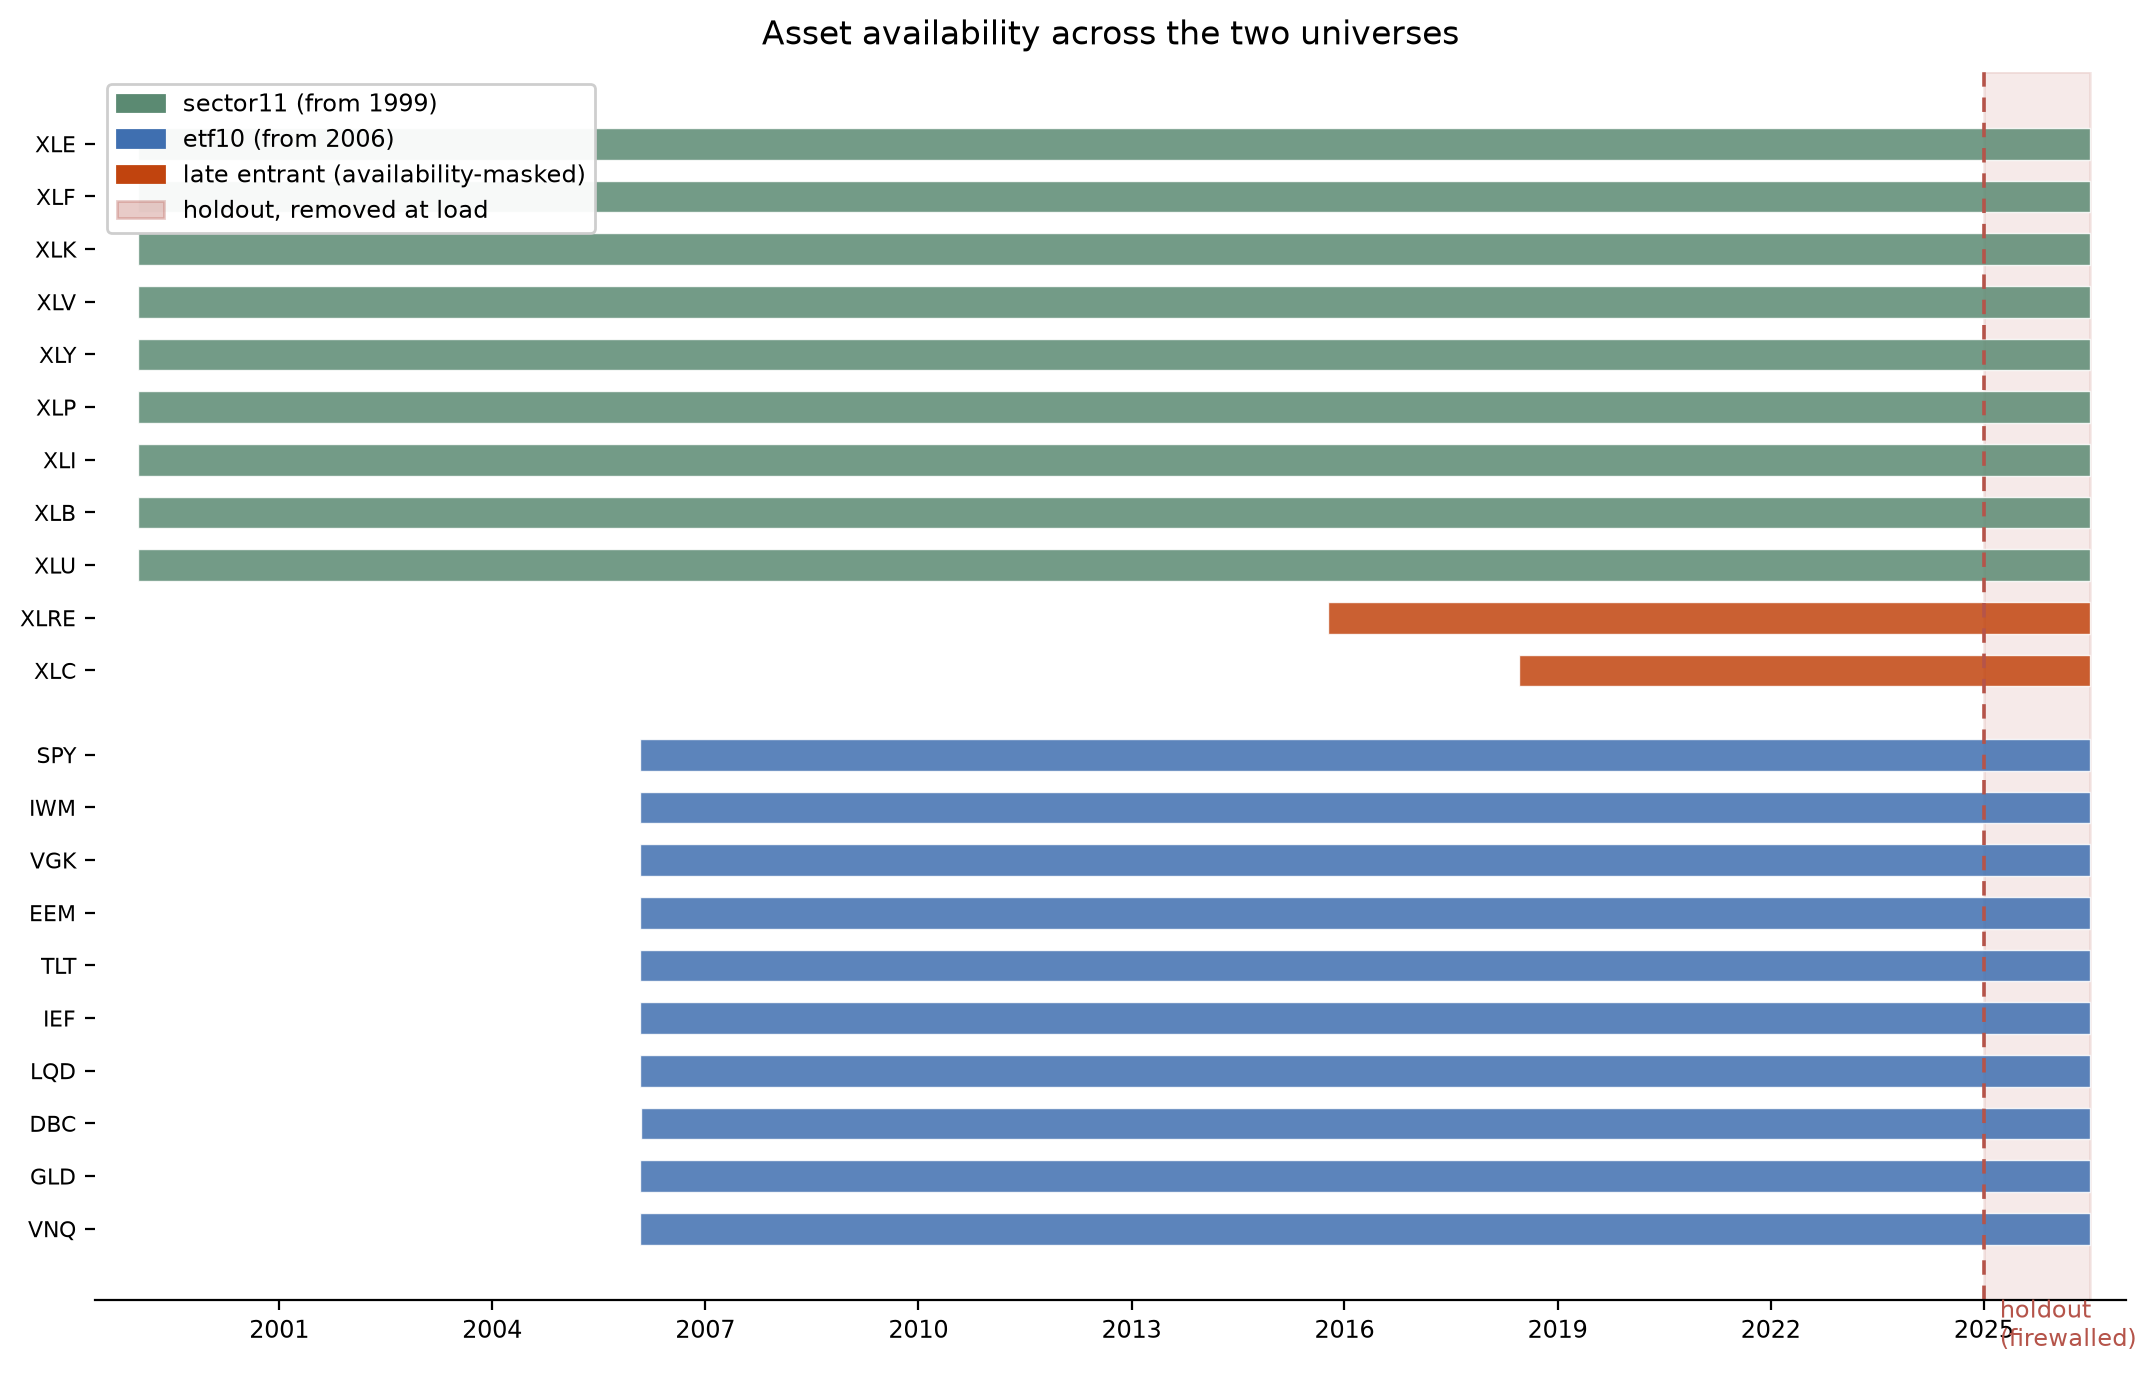
\includegraphics[width=\textwidth]{figures/fig_data_coverage.png}
  \caption[Asset availability]{Asset availability across the two universes.
  \texttt{sector11} begins in 1999 and \texttt{etf10} in 2006; XLRE and XLC enter
  late and are availability-masked until their inception. The shaded region on
  the right is the firewalled holdout, removed from every artifact at load time.}
  \label{fig:coverage}
\end{figure}

\section{Market-level signals}
\label{sec:signals}

The gating network and experts may optionally concatenate a small vector of \emph{market-level} signals to the reservoir states as input. For the gating network, since these are just additional inputs, they may or may not be used, rather than defining a regime. There are five, summarised in Table~\ref{tab:signals}. Four are drawn from FRED and one, the sentiment index, from the Federal Reserve Bank of San Francisco.

\begin{table}[t]
  \centering
  \begin{tabular}{llll}
    \hline
    Signal & Source & Lag & What it measures \\
    \hline
    VIX           & FRED \texttt{VIXCLS}          & 1 day    & Implied (expected) volatility \\
    News sentiment& SF Fed daily index            & $\ge 5$ d& Tone of economic news \\
    Term slope    & FRED \texttt{DGS10 $-$ DGS3MO}& 1 day    & Yield-curve slope \\
    Short rate    & FRED \texttt{DGS3MO}          & 1 day    & 3-month rate (policy stance) \\
    Credit spread & FRED \texttt{BAA10Y}          & 1 day    & Baa corporate credit premium \\
    \hline
  \end{tabular}
  \caption{The five market-level signals, their sources, and the publication lag
  applied before use.}
  \label{tab:signals}
\end{table}

The raw levels of these values drift enormously over the sample, thus they all are passed through the same fixed, causal pipeline. They are aligned to the trading calendar, \emph{shifted} by its publication lag, and only then standardised by a trailing $252$-day $z$-score. It's important to note that the order matters, if we standardise and then shift that can cause look-ahead leakage. The rolling statistics would be computed from values still to be published, so a $z$-score at day $t$ could depend on the future. Thus the trailing $z$-score keeps all five signals on a common, regime relevant scale. Figure~\ref{fig:signals} shows the standardised series, we can see that volatility and credit spread spike together through the 2008 and 2020 crises, similarly short rate and news sentiment show similar correlation.

\begin{figure}[t]
  \centering
  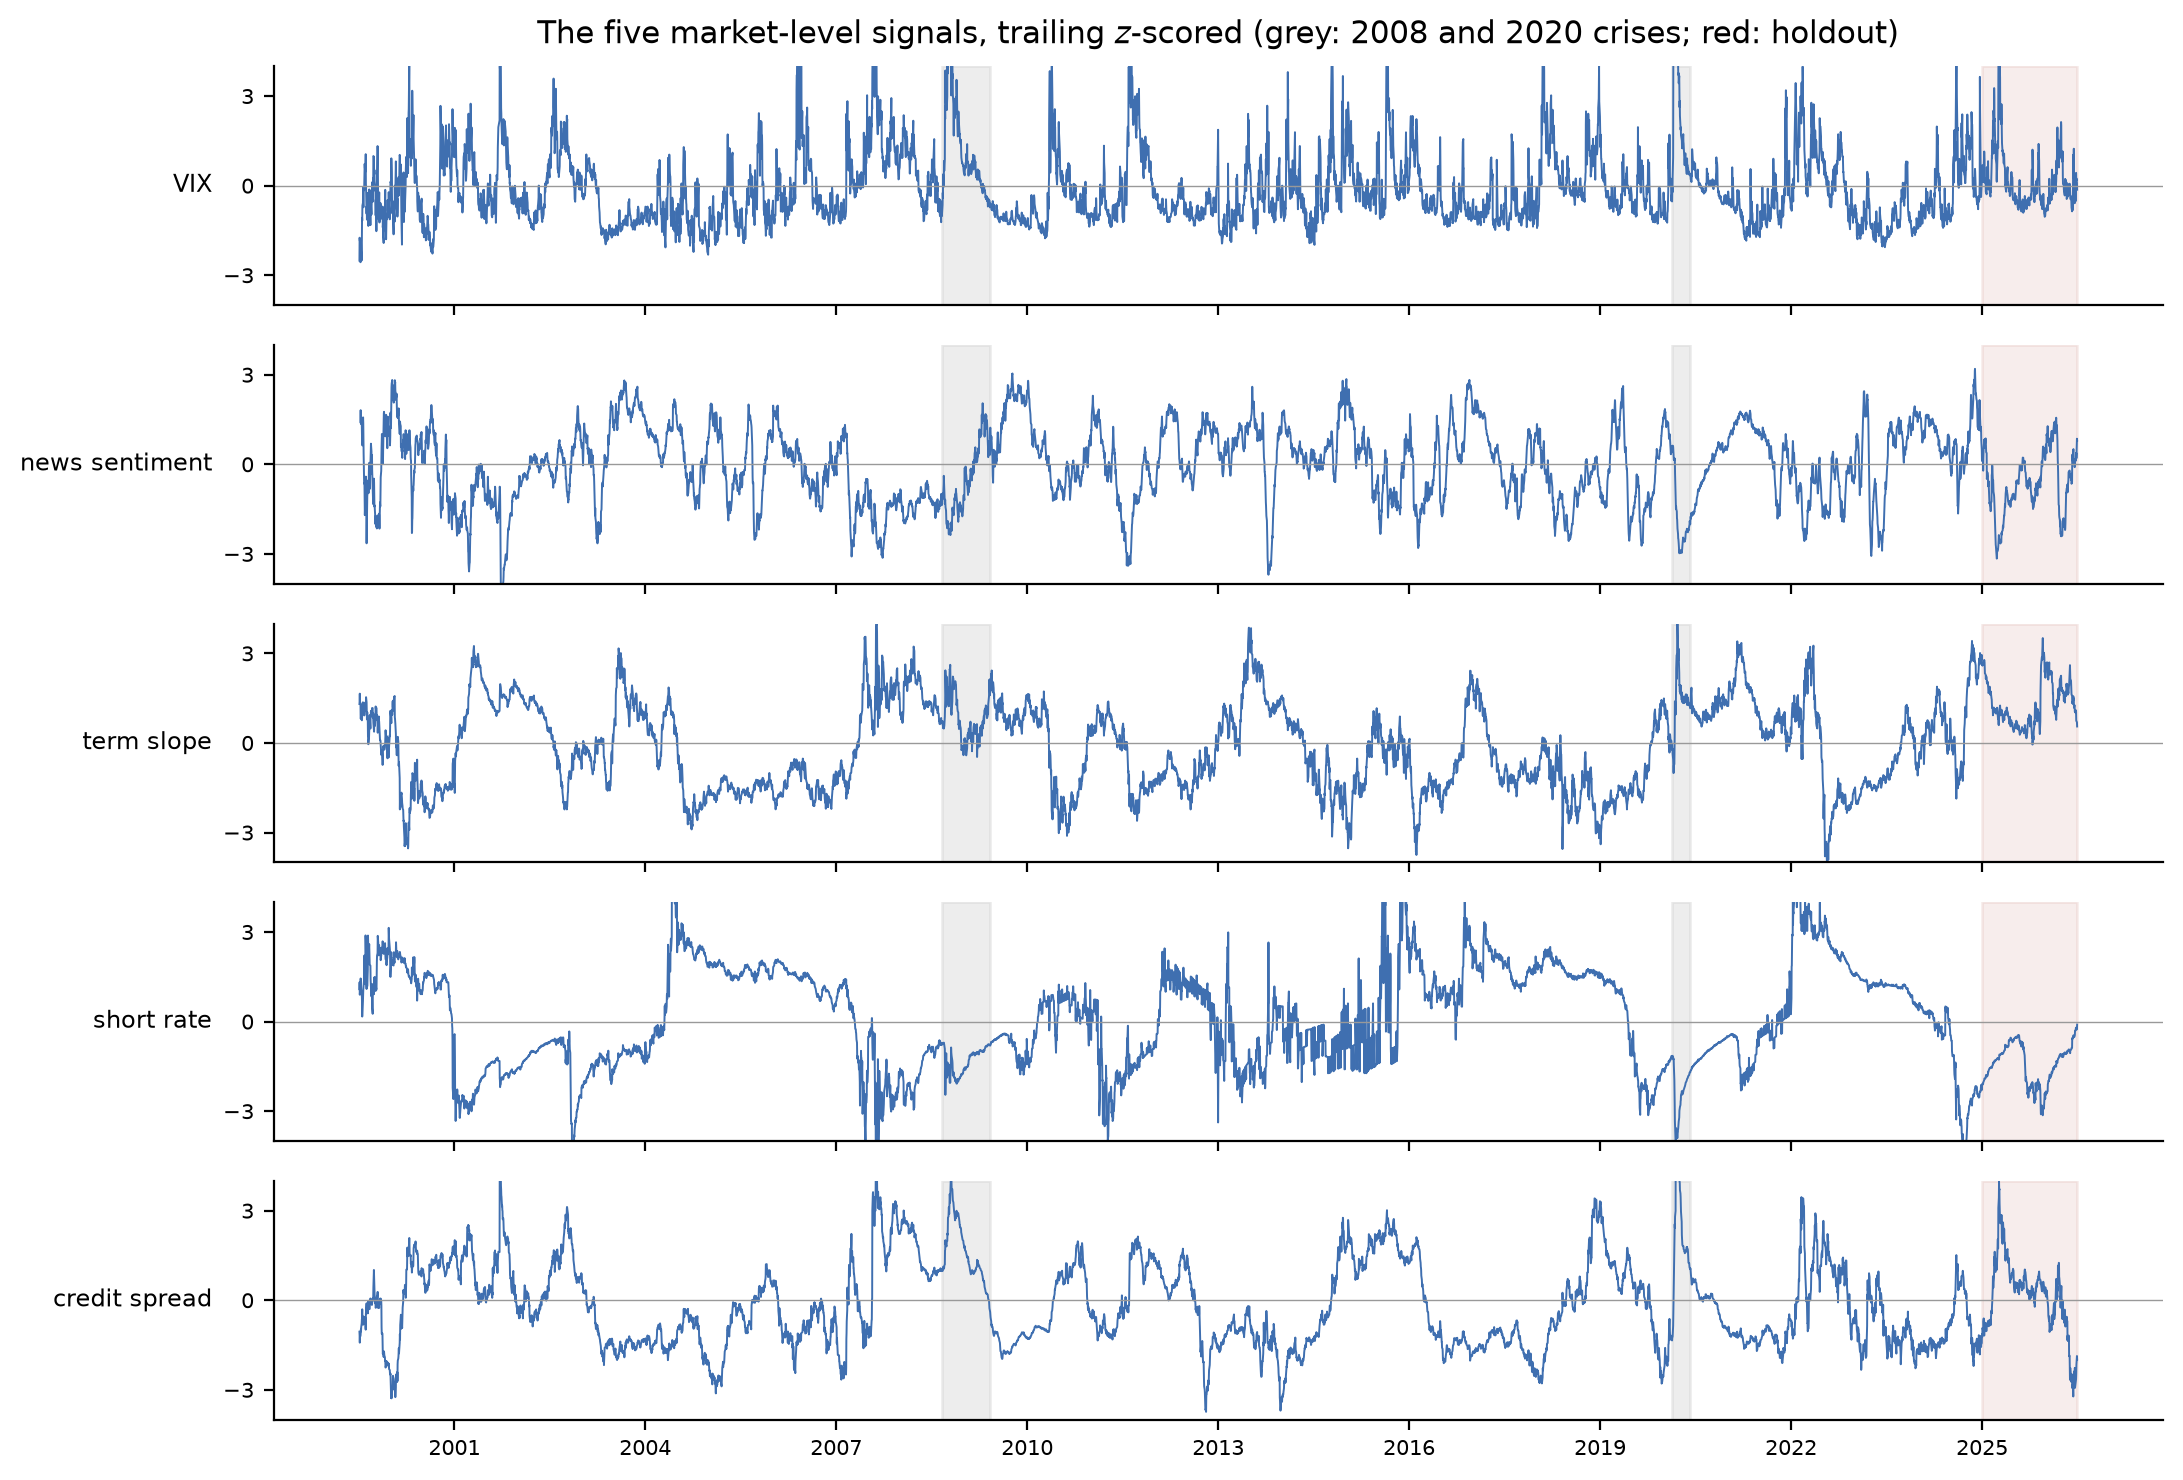
\includegraphics[width=\textwidth]{figures/fig_signals.png}
  \caption[Market-level signals]{The five market-level signals after publication
  lagging and trailing $z$-scoring. Grey bands mark the 2008 and 2020 crises; the
  red band is the firewalled holdout. Standardisation places every signal on a
  comparable, regime-relative scale.}
  \label{fig:signals}
\end{figure}

\section{Reservoir and model hyperparameters}
\label{sec:hyperparameters}

Table~\ref{tab:hyper} lists the hyperparameters, their default values I used, and the range over which I searched. As discussed in \ref{ch:methodology}, only the gate and expert head are trained. For the reservoir, I search only four hyperparameters, but as we will see in \ref{ch:results}, since no searched configuration transfer to new data, the best choice are the defaults since they carries no selection bias.



\begin{table}[t]
  \centering
  \begin{tabular}{lll}
    \hline
    Component & Hyperparameter & Value (searched range) \\
    \hline
    \multirow{4}{*}{Reservoir}
      & size $N_r$              & 300 \;(100--1200) \\
      & spectral radius $\rho$  & 0.90 \;(0.5--0.99) \\
      & leak rate $\alpha$      & 0.30 \;(0.05--1.0) \\
      & input std target        & 0.70 \;(0.3--1.5) \\
    \multirow{2}{*}{(fixed)}
      & bias scale, washout     & 0.0, \; 250 days \\
      & calibration fraction    & 0.60 \\
    \hline
    \multirow{2}{*}{Model}
      & experts $K$             & 1 (\texttt{sector11}) / 3 (\texttt{etf10}) \;(1--8) \\
      & gate temperature $\tau_g$ & 1.0 \;(0.7--1.4) \\
    \hline
    \multirow{2}{*}{Loss}
      & $\lambda_{\text{cvar}}$, $\lambda_{\text{turn}}$, $\lambda_{\text{div}}$ & 0 \\
      & $\lambda_{\text{bal}}$ (only at $K>1$)  & 0.01 \\
    \hline
    \multirow{3}{*}{Training}
      & learning rate & $3\times10^{-3}$ \\
      & max epochs   & 500\\
      & max patience     &  25 (early stopping) \\
      & gate noise $\sigma_0$ & $0.3 \to 0$ \\
      & seeds & $\{0,\dots,4\}$ \\
    \hline
  \end{tabular}
  \caption{Hyperparameters. Only the gate and experts are trained; the reservoir
  is frozen. The reported configuration is the default, not a searched winner.}
  \label{tab:hyper}
\end{table}

\section{Reproducibility}
\label{sec:reproducibility}

\paragraph{Determinism and seeds.} The code is set up so a single call seeds Python, NumPy, and PyTorch, so ``seed3'' produces the same experiment every time.  A single call seeds Python, NumPy, and PyTorch and switches on deterministic algorithms, so ``seed 3'' leads to the same experiment every time. Wherever logical, I report the final results as the mean and standard deviation over the 5 seeds $\{0,\dots,4\}$. The Simple Cycle Reservoir is deterministic, as mentioned in \ref{ch:methodology}, so it does not introduce variance across runs, and its states are cached once per configuration.

\paragraph{The variant registry.} I made a registry where the only allowed function is append. Whenever a run starts (i.e., with a different fold, split, case, etc.), it gets added to this registry. Each row records what was run, the commit, a hash of the exact configuration, and what came out (e.g., performance metrics). The configuration hash is the SHA-256 of the canonical JSON of the config, so two runs share a hash if and only if they are the same experiment, and any change to a hyperparameter produces a new hash. The entire project holds \textbf{over 3000 values} in that registry.

\paragraph{Guarding against selection.} Because the study searches over many configurations, I treat any figure obtained by picking the best as provisional until I confirm it on data outside the one used for selection. Two mechanisms provide that confirmation: first, I re-score every searched winner on folds excluded from all selection. If it does not transfer, I do not report it as a finding. Second, the firewalled holdout of Section~\ref{sec:universes} is touched exactly once, after the configuration has been frozen, and its result is reported. Together, these ensure that a result which merely reflects the amount of searching I did is caught before it reaches the conclusions.